\section*{Price Transmission Analysis}

\subsection*{Interpretation}
automate interpretation to a certain extent by learning about circumstances through online data.

\subsection*{Time Series Analysis}
Time series data has a natural temporal relation between different data points.
It is important in the analysis to extract significant temporal statistics out
of data. We will focus on analyze stationarity, autocorrelation, trend, volatility
change, and seasonality of our price datasets in R.

Stationarity of a series guarantees that the mean and variance of the data do not
change over time. This is crucial for a meaningful analysis, since if the data is
not stationary, we can not be sure that anything we derive from the present will
be consistent in the future. We can transform our data into a stationary one by
taking k-th difference to remove the underlying trend, and then apply standard
test procedures such as KPSS test [1] to see if the differenced series is stationary.

Autocorrelation is another important trait in time series data. It suggests the
degree of correlation between different time periods. By plotting correlograms
(autocorrelation plots) of our data, we will be able to identify if the fluctuation
of prices may be due to white noise or other hidden structures.

Seasonality is reasonably expected in our agricultural related time series. Several
methods might help us to detect seasonality, such as common run charts, seasonal
subseries plots, periodograms, and the correolograms we mentioned before.

(trend and volatility change is straightforward and can be concluded once we have the datasets)

[1] Kwiatkowski, D.; Phillips, P. C. B.; Schmidt, P.; Shin, Y. (1992). "Testing the null hypothesis of stationarity against the alternative of a unit root". Journal of Econometrics 54 (1–3): 159–178.


\section*{Prediction Models}
We decided to evaluate different prediction models on the processed price time series. Since the processing of the price data made available by the Indian government yielded very few usable time series we constrained ourselves to try the different prediction model on a set of \emph{daily} wholesale price series that had over 90\% support and could be sufficiently cleaned and interpolated.

\subsection*{Time Series Forecasting \footnotesize\textit{Ching-Chia Wang}}

\subsubsection*{ARMA Model}
The classical Time series forecasting approach is to use the ARMA (Auto-Regressive
Moving Average) model to predict the target variable as a linear function which
consists of the auto-regressive part (lag variables) and the moving average part
(effects from recent random shocks).

The ARMA(p,q) model: (will refine math representations later)

$Phi(B) * Y_t = Theta(B) * eps_t$

The fitting of the model and the historical
data can be accomplished by maximum likelihood estimation.

\subsubsection*{Regression}
We can also apply ARMA to the linear regression model. It is formulated as such:

$Y = Beta*X + eps,   eps ~ ARMA(p,q)$

Through OLS (Ordinary Least Squares) or GLS (General Least Squares) processes,
we can obtain an optimal Beta.

\subsection*{Feed Forward Neural Networks - Multilayer Perceptrons}
taken from M. Seeger's course on Pattern Recognition and ML

\subsection*{Recurrent Neural Networks (RNN) \footnotesize\emph{Fabian Brix}}
A recurrent neural network (RNN) is a neural network with feedback connections, enabling signals to be fed back from a layer $l$ in the network to a previous layer. As opposed to feedforward neural networks where a layer $l$ can only receive inputs from a previous layer, in an RNN the weight matrix for a layer $l$ can contain input weights from \emph{all} other neurons in the network. The simplest form of an RNN consists of an input, an output and one hidden layer as depicted in \ref{fig:simple_rnn}.
\begin{comment}
\begin{figure}
    \centering
    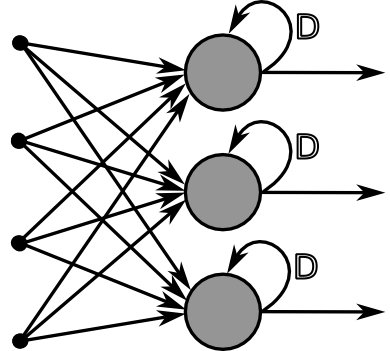
\includegraphics[width=.7\textwidth]{./img/simple_rnn.png}
    \caption{source: wikipedia}
\end{figure}
\end{comment}

\subsubsection*{General description of a discrete time RNN}
A discrete time RNN is a graph with $K$ input units $\vec{u}$, $N$ internal network units $\vec{x}$ and $L$ output units $\vec{y}$. The activation (per layer) vectors at point n in time are denoted by $\vec{u}(n) = (u_1(n),...,u_n(n))$, $\vec{x}(n) = (x_1(n),...,x_n(n))$, $\vec{y}(n) = (y_1(n),...,y_n(n))$. Edges between the units in these sets are represented by weights $\omega_{ij}\neq0$ which are gathered in adjacency matrices. There are four types of matrices:\par
\begin{itemize}
	\item $\vec{W}^{in}_{N\times K}$ contains inputs weights for an internal unit in each row respectively 
	\item $\vec{W}_{N\times N}$ contains the internal weights. This matrix is usually sparse with densities $5\%-20\%$
	\item $\vec{W}^{out}_{L\times (K+N+L)}$ contains the weights for edges, which can stem from the input, the internal units and the outputs themselves, leading to the output units.
	\item $\vec{W}^{back}_{N\times L}$ contain weights for the edges that project back from the output units to the $N$ internal units
\end{itemize}

In a \emph{fully recurrent network} every unit receives input from all other units neurons and therefore input units can have direct impact on output units. Output units can further be interconnected.\par

\paragraph{Evaluation}
The calculation of the new state of the internal neurons in time-step $n+1$ is called evaluation. 
\[
\vec{x}(n+1)=\vec{f}(\vec{W}^{in}\vec{u}(n+1)+\vec{W}\vec{x}(n)+\vec{W}^{back}\vec{y}(n))
\]
where $f=(f_1,...,f_N)$
\paragraph{Exploitation}
The output activations are then computed from the internal state of the network in the exploitation step.
\[
\vec{y}(n+1)=f^{out}(\vec{W}^{out}(\vec{u}(n+1),\vec{x}(n+1),\vec{y}(n)))
\]
where $f^{out}=(f^{out}_1,...,f^{out}_L)$ are the output activation functions and the matrix of output weights is multiplied by the concatenation of input, internal and previous output activation vectors.\par
RNNs can in theory approximate any dynamical system with chosen precision, however training them is very difficult in practice. In the following section we are going to describe our use of an RNN that exhibits exactly these properties yet is easy to train.

\subsection*{Echo State Networks}
Echo State Networks (ESN) are a type of discrete time RNNs for which training is straightforward with linear regression methods.  The temporal inputs to the network are transformed to a high-dimensional \emph{echo state}, described by the neurons of a sparsely connected \emph{random} hidden layer which is also called a reservoir. The output weights are the only weights in the network that can change and are trained in a way to match the desired output. ESNs and the related liquid state machines (LSMs) form the field of \emph{reservoir computing}.

\begin{figure}
    \centering
    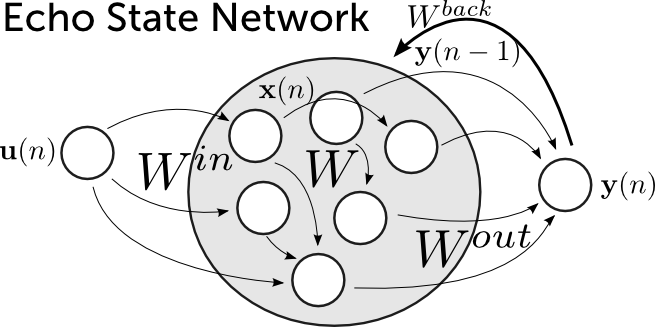
\includegraphics[width=.7\textwidth]{img/ESN_prezi.png}
    \caption{Network structure of an ESN with 1-dim. input and output}
\end{figure}

\subsubsection{Echo State Property}
The intuitive meaning of the \emph{echo state property} (ESP) is that the internal state is \textbf{uniquely} determined by the history of the input signal and the teacher forced output, given that the network has been running long enough. Teacher forcing essentially means that the output $\vec{y}(n-1)$ is forced to be equal to the next time series value $\vec{u}(n)$ and thus to the next input.
\begin{frm-def}
For every left infinite sequence $(\vec{u}(n),\vec{y}(n-1)),n=\dots,-2,-1,0$ and all state sequences $\vec{x}(n),\vec{x'}(n)$ which are generated according to
\begin{align*}	
	\vec{x}(n+1)=\vec{f}(\vec{W}^{in}\vec{u}(n+1)+\vec{W}\vec{x}(n)+\vec{W}^{back}\vec{y}(n))\\
	\vec{x'}(n+1)=\vec{f}(\vec{W}^{in}\vec{u}(n+1)+\vec{W}\vec{x'}(n)+\vec{W}^{back}\vec{y}(n))
\end{align*}
it holds true that $\vec{x}(n)=\vec{x'}(n)$ for all $n \leq 0$.
\end{frm-def}
The echo state property is ensured through the matrix of internal weights $W$

\begin{frm-thm}
Define $\sigma_{max}$ as largest singular value of $\vec{W}$, $\lambda_{max}$ as largest absolute eigenvalue of $\vec{W}$.
\begin{enumerate}
\item If $\sigma_{max} < 1$ then the ESP holds for the network
\item If $\|\lambda_{max}\| > 1$ then the network has no echo states for any input/output interval which contains the zero input/output tuple (0,0)
\end{enumerate}
\end{frm-thm}
In practice it suffices to make sure the negation of the second point holds. 

\subsubsection*{Training the ESN}
The state of the ESN is a function of the inputs it has been presented with. Each state describes an oscillator at a given time n and during training the relation between these oscillators and the output has to be learnt. Before training can be started the reservoir weights have to be normalized by the spectral radius of the weight matrix $W$. The hyperparameters are the reservoir size (dimensionality of W) and a rescale parameter of the weight matrix for slightly increasing/decreasing the spectral radius.
%http://stackoverflow.com/questions/21940860/echo-state-network-learning-mackey-glass-function-but-how

\paragraph*{Initial state determination}
Prior to training the Echo State Network has to be run for an initial set of inputs discarding the results. A spectral radius close to unity implies slow forgetting of the starting state and therefore a substantial part of the training set has to be invested. We used an initiation sequence of 740 points which equates to two years of data.

%EchoStatesTechRep.pdf, p.32
\begin{comment}
The network is run for a first set of inputs and the results are then discarded. If the spectral radius is close to unity, implying slow forgetting of the starting state, the initial set has to be a substantial part of the training dataset.
"Likewise, when the trained network is used to predict a sequence, a long initial run of the sequence must be fed into the network before the actual prediction can start. This is a nuisance because such long initial transients are in principle unnecessary"
"By contrast, a recurrent neural network such as our echo state network, but also such as the networks used in [5] need long initial runs to “tune in” to the to-be-predicted sequence. [5] tackle this problem by training a second, auxiliary “initiator” network."
\end{comment}

\paragraph*{Batch learning with Ridge Regression}
The easiest way to train an Echo State Network is through minimizing the residual of an overdetermined linear set of equations. After the reservoir initialization phase, at init\_index of the time series data, the internal states are saved together with the network inputs at every time step as rows to a matrix $X$. This results in a linear set of equations $XW^{out}=Y$, where $Y \in \mathbb{R}^N$ is the vector of outputs starting at init\_index+1. Since the system is overdetermined with no unique solution for the weights $W^{out}$ that perfectly fits all equations one applies Tikhonov regularization instead of ordinary least squares. Consequently we minimize the residual of the SLE with an added regularization term:\\
\begin{equation}
    \|XW^{out}-Y\|^2 + \|\nu W^{out}\|^2
\end{equation}
The Tikhonov regularizer allows finding a stable solution that will not adversely affect the network output by improving the conditioning of the problem. The corresponding normal equations become:
\begin{equation}
    W^{out}=(X^TX+\nu I)^{-1} X^TY
\end{equation}

\paragraph*{Teacher forcing}
Teacher forcing is the simplest training method in which the respective value of the target time series $y_{target}(n)=u(n+1)$ is fed in at every consecutive time step with input weights $W^{in}$. 

\paragraph*{Feedbacks}
During training with feedbacks the output $y(n)$ produced by the network is additionally fed back into the reservoir with feedback weights $W^{back}$. There further exists the possibility to decouple the network from the actual input during \emph{online} training which we will discuss later.

\paragraph*{Leaky integrator neurons}
\emph{Taken from Echo State Tech Rep. page 26/27}\\
% exploitation: \vec{f}(\vec{W}^{in}\vec{u}(n+1)+\vec{W}\vec{x}(n)+\vec{W}^{back}\vec{y}(n))
In order for the Echo State Network to be able to learn slowly and continuously changing dynamics and thereby to capture long-term phenomena in the price series we feed in, we need a way to introduce continuous dynamics. This is done via approximation of the differential equation of a continuous-time leaky integrator network
\begin{equation}\label{eq:leaky}
    \frac{d\vec{x}}{d\vec{t}} = C (-\alpha\vec{x} + \vec{f}(\vec{W}^{in}\vec{u}(n+1)+\vec{W}\vec{x}(n)+\vec{W}^{back}\vec{y}(n)))
\end{equation}
where C is a time constant and $\alpha$ the leaking decay rate. For the approximation we introduce a stepsize $\delta$:
\begin{equation}
    \vec{x}(n+1)=(1-\delta C \alpha) + \delta C (\vec{f}(\vec{W}^{in}\vec{u}(n+1)+\vec{W}\vec{x}(n)+\vec{W}^{back}\vec{y}(n)))
\end{equation}
In the implementation we used a simple weighted average of consecutive reservoir states $(1-\alpha)x(n-1)+\alpha x(n)$.

\begin{comment}
\begin{frm-thm}
Let a network be updated according to \eqref{eq:leaky}, with teacher-forced output.
\end{frm-thm}
\end{comment}

\paragraph*{Online learning}
In contrast to learning the weights once in batch-mode after the training run is completed one can also train the output weights in an online fashion after each consecutive presentation of an input. This method allows for a better adaption of the weights to local structures present in the data. There exist several algorithms for online training of the Echo State Networks and related reservoir networks. In the following we will shortly discuss two of the basic algorithms which are most often mentioned in academic literature. 
\begin{itemize}
\item \textbf{Least Mean Squares (LMS):} LMS algorithms try to find the optimal weights (filtered coefficients) that minimize the mean squared error for an adaptive filter which is represented by the output weights $W^{out}$ in the case of the ESN. Essentially, LMS algorithms are stochastic gradient descent methods that perform updates according to the error present at time n that update the weights according to the a priori error and a predefined constant in every iteration.\\
\indent
\begin{algorithm}[H]
\textbf{Initialization:}\\
$W^{out}(0) = \vec{0}$\\
\textbf{Update steps:}\\
\begin{enumerate}
\item $e(n) = y_{teach}-W^{out}(n-1)x(n)$
\item $W^{out}(n)=W^{out}+\mu e(n)x(n)$
\end{enumerate}
% \caption{Algo}
\end{algorithm}
\item \textbf{Recursive Least Squares (RLS):} RLS algorithms have a faster convergence speed compared to LMS algorithms. RLS optimizes the discounted square a priori error $\sum_{k=1}^{n} \lambda^{n-k}((y_{teach}(k) - y(n))^2$ with forgetting factor $\lambda$ at every timestep n. All signals generated in the sequence $1 \leq k \leq n$ are taken into account using the inverse correlation matrix of inputs P. The inputs for the adaptive filter in the case of the ESN can be the concatenation of input, generated echo states and last output.\\
\indent
\begin{algorithm}[H]
\textbf{Initialization:}\\
$\lambda < 1$\\
$P_0 = \delta I$ where $\delta \propto \sigma(input)$\\
$W^{out}(0) = \vec{0}$\\
\textbf{Update steps:}\\
\begin{enumerate}
\item $\pi(n) = P(n-1)^T \cdot x(n)$
\item $\gamma(n) = \lambda + \pi(n)x(n)$
\item $k(n) = \pi(n)/\gamma(n)$
\item $e(n) = y_{teach}-W^{out}(n-1)x(n)$
\item $W^{out}(n)=W^{out}+k(n)e(n)$
\item $P(n) = [P(n-1)-k(n)\pi(n)s]/\lambda$
\end{enumerate}
% \caption{Algo}
\end{algorithm}
The standard RLS algorithm is unstable during training, diverges when the $P(n)$ loses positive definiteness. Choosing $\lambda$ very close to 1 was temporarily enough to alleviate the problem. The QR decomposition-based RLS (QR-RLS) algorithm can, however, resolve completely this instability. Instead of working with the inverse correlation matrix of the input signal, the QR-RLS algorithm performs QR decomposition directly on the correlation matrix of the input signal. Therefore, this algorithm guarantees the property of positive definiteness and is more numerically stable than the standard RLS algorithm.
%http://zone.ni.com/reference/en-XX/help/372357A-01/lvaftconcepts/aft\_rls\_algorithms/
\end{itemize}


\paragraph*{Parameter selection with Maximum Entropy Bootstrap (Meboot)}
In order to find the best parameters for generalization during training of the neural network models with we tried to create replicate time series of a selected price sequence dataset. The method employed to this end is called 'Maximum Entropy Bootstrap' (meboot) and was introduced by H.D. Vinod in 2006. [reference]. The reason for the use of this specific method is that, due to temporal dependence, time series cannot simply be randomly sampled into a new dataset. The meboot algorithm allows for construction of random replicates of the given time series showing the same statistical properties. We did, however, not manage to fully implement the algorithm from how it was described in the paper.

\subsubsection*{Demonstration}
In this section we demonstrate the predictive power of the simplest ESN configuration with a reservoir size of 1000 neurons. Ridge Regression is used to train on and predict a time series generated using the \href{http://www.scholarpedia.org/article/Mackey-Glass_equation}{Mackey-Glass differential equation} and noise.

%\begin{subfigure}[b]{.33\textwidth}
%\centering
%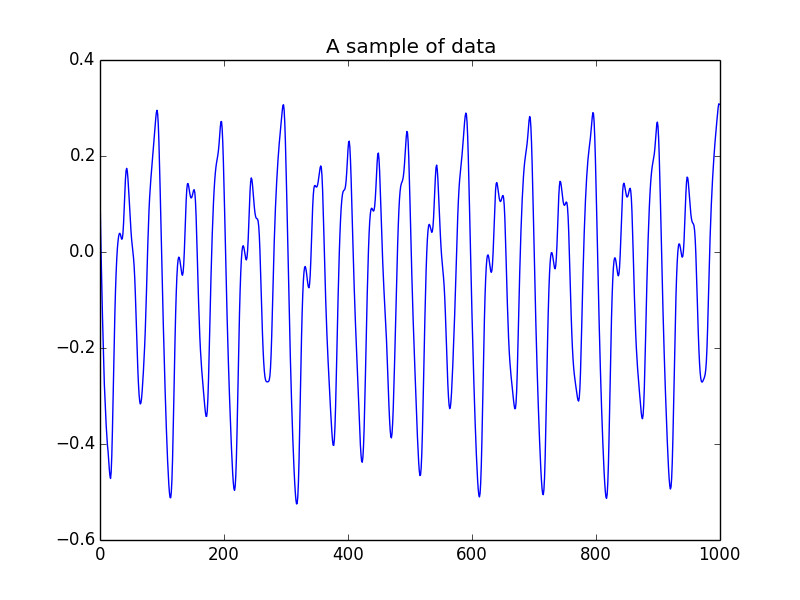
\includegraphics[width=\textwidth]{./img/plots/esn/mg/data1000.png}
%\caption{Sample of 1000 training points of Mackey Glass series}
%\label{subfig:mg_train}
%\end{subfigure}

\begin{figure}[!ht]
    \centering
        \begin{subfigure}[b]{.45\textwidth}
        \centering
        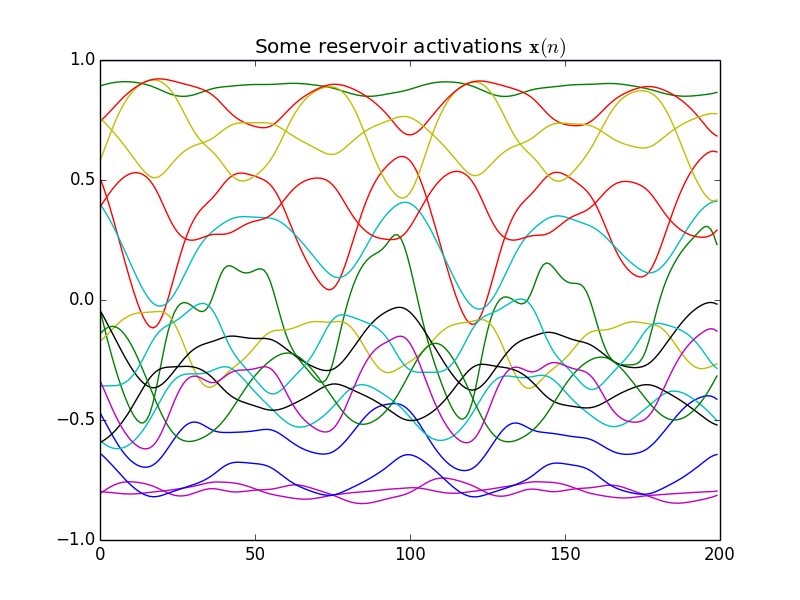
\includegraphics[width=\textwidth]{./img/plots/esn/mg/resact.png}
        \caption{Sample of ESN activations resulting from the training series}
        \label{subfig:mg_act}
        \end{subfigure}
        \quad 
        \begin{subfigure}[b]{.45\textwidth}
        \centering
        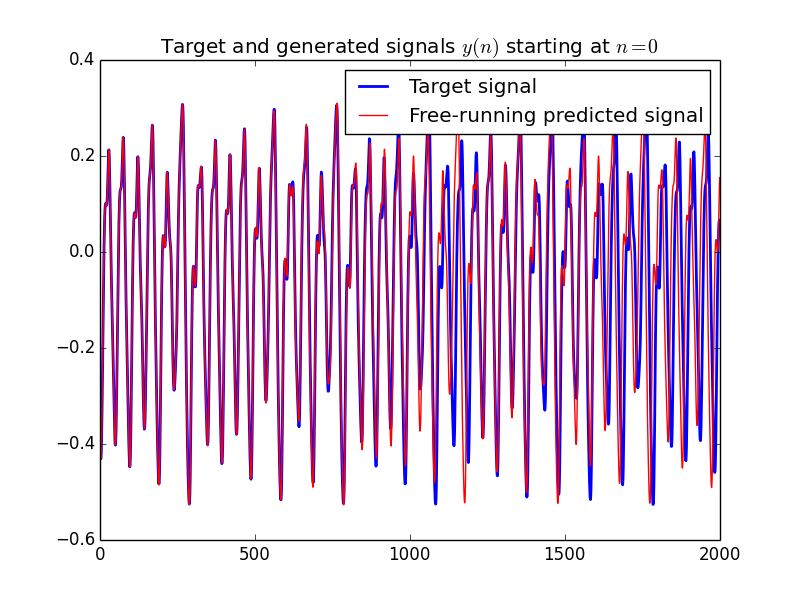
\includegraphics[width=\textwidth]{./img/plots/esn/mg/pred1000_br.png}
        \caption{Near perfect prediction 1000 points Mackey Glass testset by ESN}
        \label{subfig:mg_pred}
        \end{subfigure}
    \caption{Results of simple ESN trained with Ridge Regression on a Mackey Glass time series consisting of 2000 points; parameters: spectral radius $1.25$, leaking rate $0.3$.}
    \label{fig:mackeyglass}
\end{figure}

\subsubsection*{Obtained results}
The mackey glass time series is generated by a function with added noise. Since the development of commodity prices doesn't follow a similarly easily describable pattern we did not expect to obtain comparable results. Once trained on several years of price series data the ESN is capable of predicting prices very accurately on a day-to-day basis without any need for retraining. However, due to the limited usefulness of day-to-day predictions, we would like to predict prices farther into the future with relative accuracy. So far we have only achieved predicting the general trend for 6 to 7 days and we are not sure if greater accuracy is achievable with these models. Our experiments with inputting additional data like temperature, precipitation, consumer price index (inflation) and twitter data show NO? significant improvements. 

% NO BLANK SPACES
\begin{figure}[!ht]
    \centering
        \begin{subfigure}[b]{.45\linewidth}
        \centering
        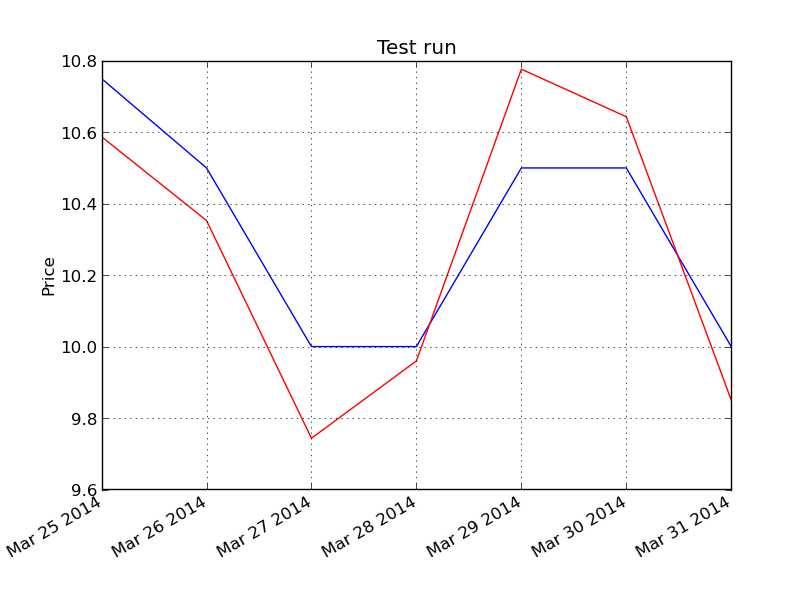
\includegraphics[width=\textwidth]{./img/plots/esn/daily/gujarat_potato_online_7d_1d.png}
        \caption{Wholesale price of potato, state Gujarat; test RMSE in rupees: 0.199} 
        \label{subfig:res_7d_1}
        \end{subfigure}
        \quad
        \begin{subfigure}[b]{.45\linewidth}
        \centering
        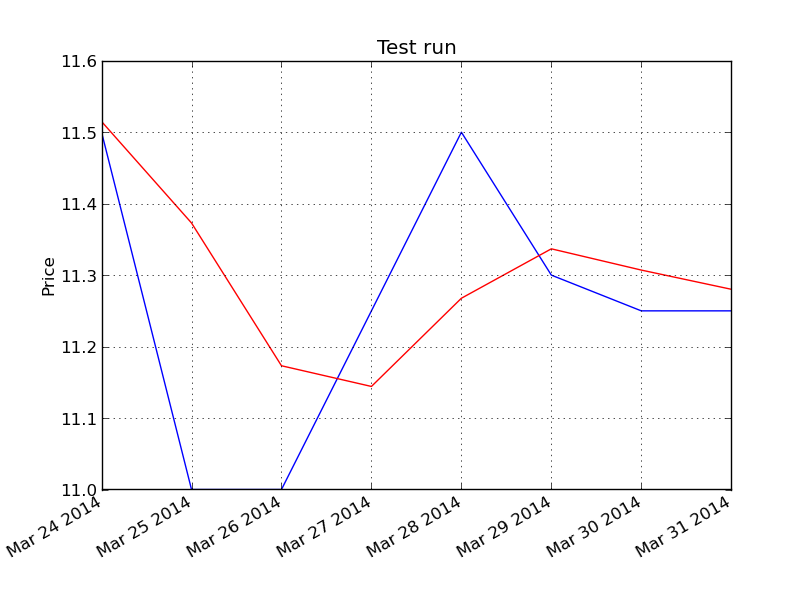
\includegraphics[width=\textwidth]{./img/plots/esn/daily/uttar_pradesh_redonion_7d_1d.png}
        \caption{Wholesale price of red onion, state Uttar Pradesh; test RMSE in rupees 0.145}
        \label{subfig:res_7d_2}
        \end{subfigure}
    \caption{7 day day-to-day prediction for two different commodities in different states}   
    \label{fig:res_7d}
\end{figure}

\begin{figure}[!ht]
    \centering
        \begin{subfigure}[b]{.45\textwidth}
        \centering
        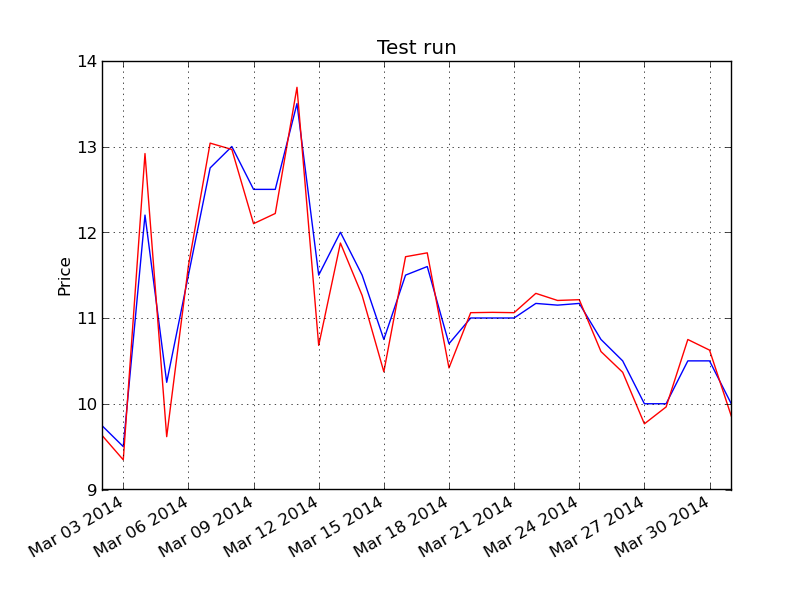
\includegraphics[width=\textwidth]{./img/plots/esn/daily/gujarat_potato_online_30d_1d.png}
        \caption{Wholesale price of potato, state Gujarat; test RMSE in rupees: 0.293} 
        \label{subfig:res_30d_1}
        \end{subfigure}
        \quad
        \begin{subfigure}[b]{.45\textwidth}
        \centering
        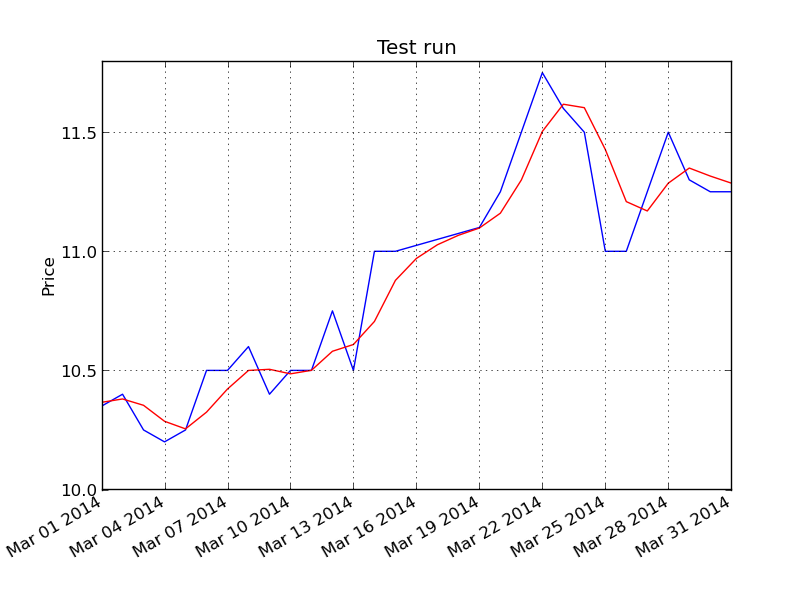
\includegraphics[width=\textwidth]{./img/plots/esn/daily/uttar_pradesh_redonion_30d_1d.png}
        \caption{Wholesale price of red onion, state Uttar Pradesh; test RMSE in rupees 0.145}
        \label{subfig:res_30d_2}
        \end{subfigure}
    \caption{30 day day-to-day prediction for two different commodities in different states}   
    \label{fig:res_30d}
\end{figure}

\begin{figure}[!ht]
    \centering
        \begin{subfigure}[b]{.45\textwidth}
        \centering
        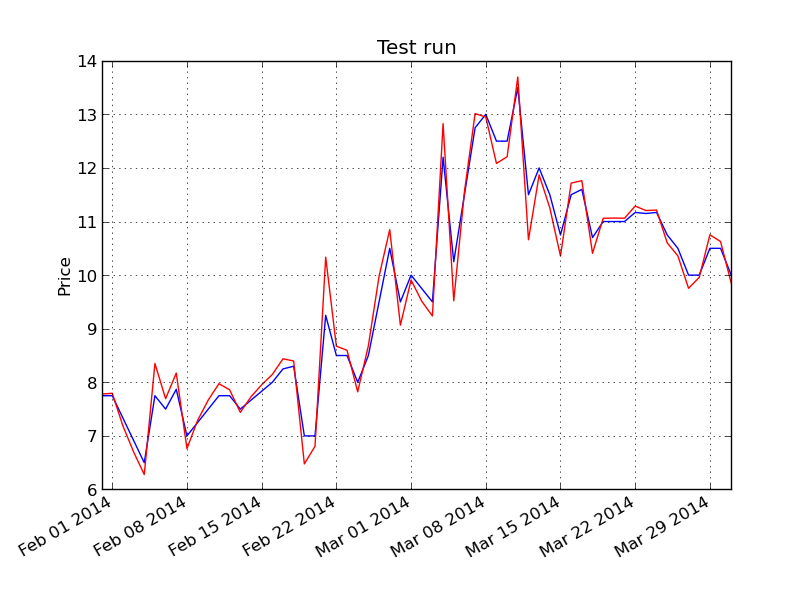
\includegraphics[width=\textwidth]{./img/plots/esn/daily/gujarat_potato_online_60d_1d.png}
        \caption{Wholesale price of potato, state Gujarat; test RMSE in rupees: 0.310} 
        \label{subfig:res_60d_1}
        \end{subfigure}
        \quad
        \begin{subfigure}[b]{.45\textwidth}
        \centering
        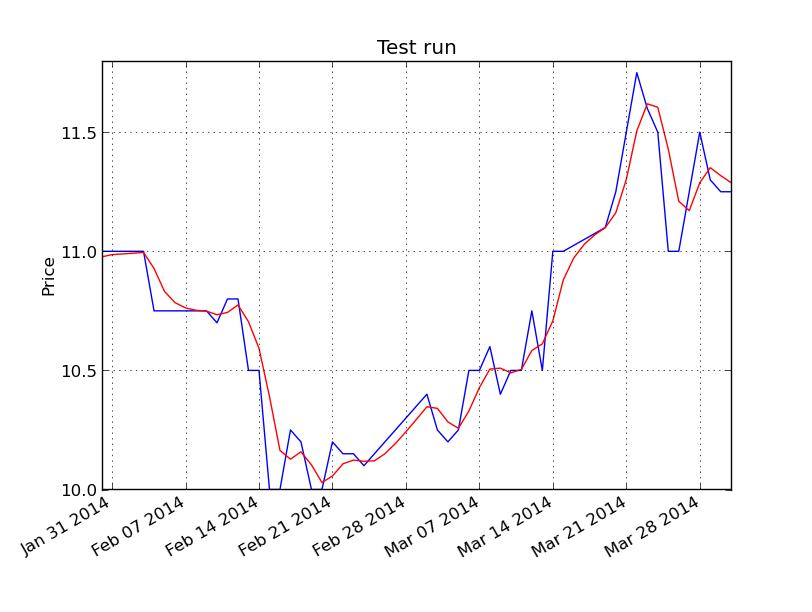
\includegraphics[width=\textwidth]{./img/plots/esn/daily/uttar_pradesh_redonion_60d_1d.png}
        \caption{Wholesale price of red onion, state Uttar Pradesh; test RMSE in rupees 0.127}
        \label{subfig:res_60d_2}
        \end{subfigure}

    \caption{60 day day-to-day prediction}   
    \label{fig:res_60d}
\end{figure}

Adjusted for inflation the prices mostly lose their upwards trend and should become easier for the network to predict. This is the case, but good predictions are obtained more by chance by selecting subsets of a series to train on because modeling the dynamics of the whole series seems to be too complex for the network. In their current state, due to very limited amounts of available data, the twitter indicators cannot prove their use. Significantly bolstered however they would offer a wide range of possibilities. Matching these indicators to available price data series could show up relationships between conversations and the actual price. These relationships could be used to track price changes in real-time on a regional level through the conversations on twitter and thereby prove an interesting alternative to the inadequate/flawed data monitoring of governments. Improving predictions if possible would certainly acquire a lot more focused research in the area recurrent neural networks for time series prediction. The Echo State Network was implemented from scratch in scientific python.

\subsubsection*{Further ESN research}
Further research concerning the stability of online training of the ESN and its predictability power would encompass the implementation of a stable RLS algorithm such as the Inverse QR-RLS as well as the implementation of the Backpropagation and Decorrelation (BPDC). The latter does not require a specific set up of the network rendering concerns about the initialization run and the spectral radius of the weight matrix void. Using these algorithms a performance analysis of the network has to be done before we can test the influence of additional inputs. Maybe research into Linear System Theory can provide answers as to how to make the network responsive to its own inputs in the generative run. It would lastly be interesting  to compare the ESN to its "rival" the Long Short Term Memory Network trained with the Evolino method.
ADD REFERENCES

\subsection*{Data Mining}
\emph{Alexander Buesser} \\

In this section we give a brief introduction to association rule mining and detail the implementation and evaluation of the system. In order to run the code you will need to install the libraries Scipy and Orange.

\subsubsection{A brief introduction to Association rule mining}

The objective of association  mining is the elicitation of useful rules from which new knowledge can be derived. Association mining applications have been applied to many different domains including market basket analysis, risk analysis in commercial environments, clinical medicine and crime prevention. They are all areas in which the relationship between objects can provide useful knowledge. 

Itemsets are identified by the use of two metrics support and confidence. 

Support is a measure of the statistical significance of the rule. Rules with a very low support are more likely to occur by chance. With respect to the market basket analysis items that are seldom bought together by customers are not profitable to promote together. For this reason support is often used as a filter to eliminate uninteresting rules. 

Confidence on the other hand is is a measure on how reliable the inference made by a rule is. For a given rule $A \implies B$, the higher the confidence, the more likely it is for the item set B to be present in the transactions that contain A. IN a sense confidence provides an estimate of the conditional probability for B given A. 

It is worth noting that the inference made by an association rule does not necessarily imply causality. Instead the implication indicates a strong concurrence relationship between items in the antecedent and consequent of the rule. 

So how do we go about implementing this in an algorithm? A rather naive approach would be to check if each itemset satisfies minimum support. However this is rather inefficient and unnecessary. We can make use of of the observation that every subset of a frequent item set also has to be a frequent item set. This works the other way as well. If a set is not frequent then its superset can not be frequent either. This observation allows us to prevent unnecessary computation. The Apriori Algorithm uses this downward closure to identify frequent item sets. Candidates that do not satisfy minimal support are pruned, which automatically reduces the algorithm's search space. Once frequent item sets have been generated the algorithm enters the second face, namely generating derivations for which the metric minimal confidence is used. 

\subsubsection{Implementation}

The implementation is guided through three stage namely data crunching, classification and  mining where the later is a straight forward implementation of the mining library orange. \\



In order to run the Apriori Algorithm we needed to do some preprocessing since the data available was in an incompatible format. The data readily available to us was in the form 
of Date Country City Category Commodity 1, Date Country City Category Commodity 2. In the statistics community this kind of format is referred to as the "long format". In order to run Apriori we need to convert the table to a "wide format" meaning that all commodities need to be related to one index. You can imagine a matrix where the y axis is described by city + date and the x axis is labeled with all the available commodities. To do the conversion we used Stata, a statistical software which is mostly used in the field of social science. Before reading the data into state we filtered the document for special characters ("", /) and replaced all unavailable price informations with "NA". For this purpose we used the filter.py script. Once we read in the data into state we removed duplicates and started the conversion. To reproduce the correct table format you fan follow our implementation in the stata script.  The data is now in the correct table format what remains to be done is slicing the table according to a city and sorting the data in order of decreasing time stamps. These steps are performed in the dataFrame.py. We now continue to process the files by classifying continues variables into categories. We therefor filtered the maximum and minimum increase/decrease in price to establish a range of values. Depending on whether a price increase fall into the first, second or third of the price range we classified it as small, medium or big increase/decrease respectively. The categorical data can now be processed by the assoc.py file. The library orange provides an implementation of the a priori gen algorithm. We simply set the min support value and write the 10 rules with the highest support count to a file. 

\subsubsection{Results}

What we were hoping to find were seasonal related price changes such as those we experience when shopping for fruits and vegetables at our local grocery stores. Rules such as $Tomatoes = big increase \implies potatoes = small decrease$ could serve 


Our initial granularity was set to weekly data. From our meta analysis we observed that prices quite frequently stay unchanged over the period of several weeks. This resulted in an overwhelming amount of rules in the form of commodity $A = unchanged \implies B= unchanged$. This made it really hard to filter the set for insightful rules. We therefor decided to compare price changes over the period of 12 weeks. Although the majority of the rules still remained in the above form we managed to extract some relations related to price changes. 

We conclude that the strongest correlations exist between commodities with unchanged prices. This observation underlines the nature of food commodities. Agricultural commodities are known to be less volatile then for example energy commodities. We further noticed that depending on the region we would have a totally different rule count. Capital cities tend to have a bigger rule base meaning that there exist a higher correlation between products. Two extreme example are Dassau, which resulted in no patterns at all and Shillong which produced over 260000 rules. In addition our experiments showed the finer the granularity of the data the higher the support and correlation between products. This is only natural given that prices can stay stable over the period of weeks or even months. 

\subsubsection{Trading advice }

As concluded above our algorithm found many associations between products. In order to interpret most of the results specialized domain knowledge in trading with commodities is  necessary. Some more obvious rules we managed to interpret were the following:

$BreadLocal=big increase MilkCowBuffalo=unchanged increase \implies \\MaidaNA=unchanged increase$. If prices of bread inflate it is save to trade Maida, as its price will most certainly stay stable. \\$BiscuitGlucose=unchanged increase \implies BesanNA=small increase$, similarly means that stable pries in biscuits will imply a small increase in Besan. 

\begin{comment}
\subsubsection*{Finding the right topology for the specific prediction problem}

\subsubsection*{Converge}
conceive network that converges fast to speed up training\par
"Known supervised training techniques for RNNS comprise Back Propagation Through Time (BPTT), Real Time Recurrent Learn- ing (RTRL) or Extended Kalman Filtering (EKF) all of which have some major drawbacks."
{\em Application of BPTT to RNNs requires stacking identical copies of the network thus unfolding the cyclic paths in the synaptic connections. Unlike back-propagation used in feed-forward nets, BPTT is not guaranteed to con- verge to a local error minimum, computational cost is O(TN2) per time step where N is the number of nodes, T the number of epochs. In contrast RTRL needs O((N + L)4) (L denotes number of output units), which makes this algorithm only applicable for small nets. The algorithm complexity of EKF is O(LN2). EKF is mathematically very elaborate and only a few experts have trained predefined dynamical system behaviors successfully}\par

\cite{jaeger_echo_state_RNN}
The third section explains how echo state networks can be trained in a
supervised way. The natural approach here is to adapt only the weights
of network-to-output connections. Essentially, this trains readout functions
which transform the echo state into the desired output signal. Technically,
this amounts to a linear regression task.
\end{comment}


